\documentclass{exam}
\usepackage[utf8]{inputenc}
\usepackage{lmodern}
\usepackage{microtype}

% \usepackage[parfill]{parskip}
\usepackage[dvipsnames]{xcolor}
\usepackage{amsmath}
\usepackage{amsfonts}
\usepackage{amsthm}
\usepackage{siunitx}
\DeclareSIUnit\year{yr}
\DeclareSIUnit\foot{ft}
\DeclareSIUnit\litre{\liter}

\usepackage{skull}

\usepackage{pgfplots}
\usepgfplotslibrary{polar}
\pgfplotsset{compat=1.11}
\usepgfplotslibrary{statistics}
\usepackage{graphicx}
\usepackage{sidecap}
\sidecaptionvpos{figure}{c}
\usepackage{float}
\usepackage{gensymb}
\usepackage{tkz-euclide}
\usetkzobj{all}
\usepackage{commath}
\usepackage{hyperref}
\usepackage{enumitem}
\usepackage{wasysym}
\usepackage{multicol}
\usepackage{mathtools}
\usepackage{tcolorbox}
\usepackage{tabularx}
\usepackage[version=4]{mhchem}
\usepackage{changepage}
\usepackage{listings}
\lstset{basicstyle=\ttfamily\linespread{0.8}\small}

\renewcommand*{\thefootnote}{\fnsymbol{footnote}}

\newtheorem*{thm}{Theorem}
\newtheorem*{iden}{Identity}
\newtheorem*{lemma}{Lemma}
\newtheorem{obs}{Observation}
\theoremstyle{definition}
\newtheorem*{defn}{Definition}
\newtheorem*{ex}{Example}
\newtheorem{con}{Construction}
\newtheorem*{alg}{Algorithm}

\newtheoremstyle{break}
  {\topsep}{\topsep}%
  {\itshape}{}%
  {\bfseries}{}%
  {\newline}{}%
\theoremstyle{break}
\newtheorem*{bthm}{Theorem}

% russian integral
\usepackage{scalerel}
\DeclareMathOperator*{\rint}{\scalerel*{\rotatebox{17}{$\!\int\!$}}{\int}}

% \DeclareMathOperator*{\rint}{\int}

\pgfplotsset{vasymptote/.style={
    before end axis/.append code={
        \draw[densely dashed] ({rel axis cs:0,0} -| {axis cs:#1,0})
        -- ({rel axis cs:0,1} -| {axis cs:#1,0});
    }
}}

% \pointsinrightmargin
\boxedpoints
\pointname{}

\newcommand{\questioA}{\question[\texttt{\textbf{\color{Cerulean} A}}]}
\newcommand{\questioM}{\question[\texttt{\textbf{\color{PineGreen} M}}]}
\newcommand{\questioE}{\question[\texttt{\textbf{\color{WildStrawberry} E}}]}
\newcommand{\questioS}{\question[\texttt{\textbf{\color{Goldenrod} S}}]}
\newcommand{\questioO}{\question[\texttt{\textbf{\color{BurntOrange} O}}]}

\newcommand{\parA}{\part[\texttt{\textbf{\color{Cerulean} A}}]}
\newcommand{\parM}{\part[\texttt{\textbf{\color{PineGreen} M}}]}
\newcommand{\parE}{\part[\texttt{\textbf{\color{WildStrawberry} E}}]}
\newcommand{\parS}{\part[\texttt{\textbf{\color{Goldenrod} S}}]}
\newcommand{\parO}{\part[\texttt{\textbf{\color{BurntOrange} O}}]}

\newcommand{\subparA}{\subpart[\texttt{\textbf{\color{Cerulean} A}}]}
\newcommand{\subparM}{\subpart[\texttt{\textbf{\color{PineGreen} M}}]}
\newcommand{\subparE}{\subpart[\texttt{\textbf{\color{WildStrawberry} E}}]}
\newcommand{\subparS}{\subpart[\texttt{\textbf{\color{Goldenrod} S}}]}
\newcommand{\subparO}{\subpart[\texttt{\textbf{\color{BurntOrange} O}}]}

\newcommand{\mainHeader}[2]{\section*{NCEA Level 2 Mathematics\\#1. #2}}
\newcommand{\mainHeaderHw}[2]{\section*{NCEA Level 2 Mathematics (Homework)\\#1. #2}}
\newcommand{\seealso}[1]{\begin{center}\emph{See also #1.}\end{center}}
\newcommand{\drills}[1]{\begin{center}\emph{Drill problems: #1.}\end{center}}
\newcommand{\basedon}[1]{\begin{center}\emph{Notes largely based on #1.}\end{center}}

\begin{document}

\mainHeaderIntg{16}{Anti-differentiation}
A few weeks ago when we looked at kinematics, I hinted that finding area was in some way the inverse to finding slope. In last
week's questions, the curtain was pulled back a little further when we calculated an area function for a variable endpoint, took
the derivative, and got the original function back. Next week, all will be revealed; but first, we need to do a little bit more
work. This week, we're going to look at \textit{anti-differentiation}: finding the original function given its derivative.

\begin{ex}
  One antiderivative of $ y' = 3x^2 + 4 $ is $ x^3 + 4x $. Another is $ x^3 + 4x + 1 $. A third is $ x^3 + 4x + 7 $. Obviously
  every function of the form $ y = x^3 + 4x + C $ for some constant $ C $ will differentiate to the given $ y' $, so we must remember
  always to make this clear.
\end{ex}

We also call antiderivatives \textbf{indefinite integrals}, and in this notation the above example is
\begin{displaymath}
  \rint 3x^2 + 4 \dif{x} = x^3 + 4x + C.
\end{displaymath}

\begin{ex}
  The most general antiderivative of $ \sin x $ is $ -\cos x + C $.
\end{ex}

\begin{ex}
  The most general antiderivative of $ \tan x $ is $ -\ln \abs{\cos x} + C $.
\end{ex}

\begin{ex}
  $ \rint \frac{1}{x + 3} \dif{x} = \ln \abs{x + 3} + C $.
\end{ex}

\begin{ex}
  $ \rint \tan^2 \theta \dif{\theta} = \rint \sec^2 \theta - 1 \dif{\theta} = \tan \theta - \theta + C $.
\end{ex}

\begin{ex}
  $ \rint \frac{2x}{x^2 + 1} \dif{x} = \ln \abs{x^2 + 1} + C $.
\end{ex}

\begin{ex}
  $ \rint Ke^{Kx} \dif{x} = e^{Kx} + C $ for all constants $ K $.
\end{ex}

\subsection*{Questions}
\begin{questions}
  \questioA In each case, find the most general antiderivative.
    \begin{parts}
      \part $ f(x) = 2x $
      \part $ f(x) = x^{-3} $
      \part $ f(x) = 0 $
      \part $ f(x) = \sec^2 (x) + \sqrt{x} $
      \part $ f(x) = x\sqrt{x} $
      \part $ f(t) = \sin t - \cos t $
    \end{parts}
  \questioA Verify the above examples by differentiation.
  \questioA Show that $ \rint 3x^2 + 4x + 5 + 2e^{2x} \dif{x} = x^3 + 2x^2 + 5x + e^{2x} + C $.
  \questioA Find $ y' $ when $ y = 3 + \sin (2x + 4) $ and hence find $ \rint 2 \cos(2x + 4) \dif{x} $.
  \questioA If $ \od{y}{t} = 1.5 \sqrt{t} $ and $ y(4) = 10 $, find $ y(t) $ exactly.
  \questioM Find $ f $ if $ f''(x) = 12x^2 + 6x - 4 $, $ f(0) = 4 $, $ f(1) = 1 $.
  \questioA The velocity of a particle is given by $ v(t) = 2t + 1 $. Find its position at $ t = 4 $
            if its position at $ t = 0 $ is $ x = 0 $.
  \questioM The acceleration of a particle is given by $ a(t) = 10\sin t + 3\cos t $. At $ t = 0 $, its position is $ x = 0 $; at $ t = 2\pi $,
            its position is $ x = 12 $. Find its position at $ t = \frac{\pi}{2} $.
  \questioA Find all functions $ g $ such that $ g'(x) = 4 \sin x + \frac{2x^5 - \sqrt{x}}{x} $.
  \clearpage
  \questioM For each function, sketch an antiderivative passing through $ (0, 0) $:

    \begin{center}
      \begin{tabular}{cc}
        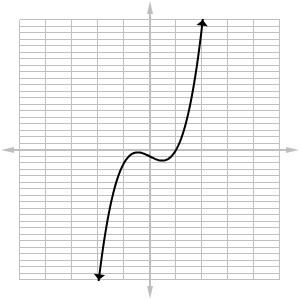
\includegraphics[width=0.4\textwidth]{anti1}&
        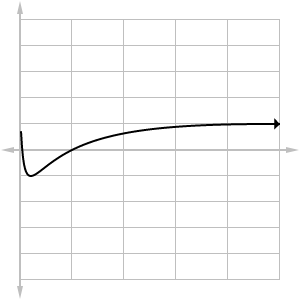
\includegraphics[width=0.4\textwidth]{anti2}\\
        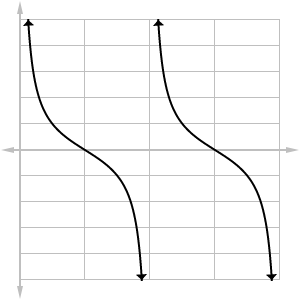
\includegraphics[width=0.4\textwidth]{anti3}&
        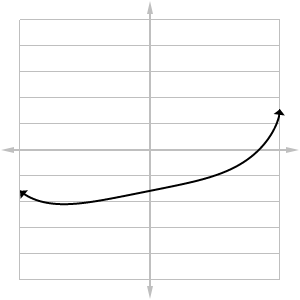
\includegraphics[width=0.4\textwidth]{anti4}\\
        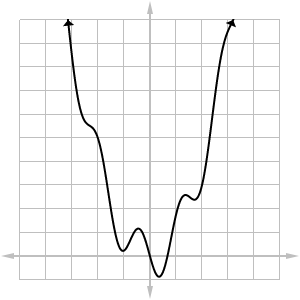
\includegraphics[width=0.4\textwidth]{anti5}&
        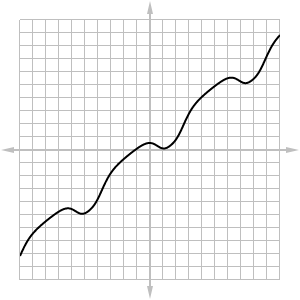
\includegraphics[width=0.4\textwidth]{anti6}
      \end{tabular}
    \end{center}
\end{questions}

\end{document}
